\chapter{Acerca de Quadriga}\label{cap.quadriga}
\section{Introducción}
El corazón de \textit{5Gneralife} está basado en \textit{QuaDRiGa} en su totalidad, por lo que resulta conveniente conocer previamente su funcionamiento y sus nociones básicas antes de detenerse a detallar la implementación del simulador en sí.

\textit{QUAsi Deterministic RadIo channel GenerAtor, QuaDRiGa} es un proyecto cuya finalidad es facilitar el desarrollo de simuladores de redes móviles de nivel de sistema, gracias a su función, que no es otra que generar respuestas impulsivas realistas para distintos canales de radio modelados de acuerdo a diversos estándares. En concreto, en su última versión hasta la fecha (v2.0), \textit{QuaDRiGa} integra un total de 78 modelos de canal, incluidos modelos de acuerdo a estándares creados por diversas entidades como 3GPP o WiNNER \cite{winner} o mmMAGIC.

Aunque \textit{QuaDRiGa} fue concebido para su uso en LTE, las actualizaciones más recientes han hecho compatible su uso con simulaciones orientadas a 5G mediante implementaciones como un rango más amplio de frecuencias, integración de MIMO en las antenas o inclusión de modelos de \textit{small cells} para los distintos entornos.

En este capítulo se especificarán sus principales características y especificaciones, así como su estructura de programación y su modo de uso.

\section{Características}

Puesto que \textit{QuaDRiGa} no pretende ser un simulador independiente, sino un recurso del que se pueden servir otros simuladores como el que ha sido desarrollado, no integra funcionalidades típicas de simuladores como datos característicos del entorno simulado.

Teniendo esto en cuenta, entre sus características generales, podemos destacar:

\begin{itemize}
    \item Permite configuración libre de capas de red con varios transmisores y receptores.
    \item Posibilidad de crear enlaces MIMO.
    \item Su rango de frecuencias es de 450 MHz hasta 100 GHz.
    \item Modela la evolución en el tiempo de sus elementos incluyendo parámetros de pequeña y gran escala.
    \item Modela escenarios rurales y urbanos, interiores y exteriores, todos ellos incluyendo los casos con visión directa (LOS) y sin visión directa (NLOS), con posibilidad de transición entre ellos por parte de los usuarios. Para estos modelos se hace uso de los parámetros establecidos por WINNER+ y por 3GPP-3D.
    \item Implementación completa para Matlab, con programación orientada a objetos. Compatibilidad con algunas versiones de Octave.
\end{itemize}

Una de las características más interesantes y que caracteriza a \textit{QuaDRiGa} es la posibilidad de implantación de distintos tipos de escenario en una misma simulación. Esta funcionalidad pretende modelar el comportamiento de un usuario que se encuentra en movimiento, ya sea a pie o en vehículo, ya que las condiciones de su entorno cambian constantemente a lo largo del recorrido.

\begin{figure}[h!]
	\centering
    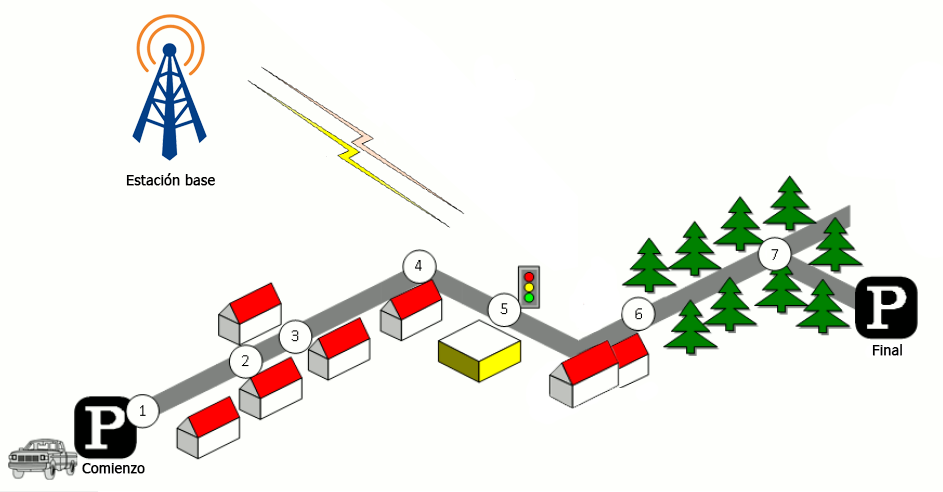
\includegraphics[width=\linewidth]{imagenes/transiciones.png}
	\caption{Ilustración de un entorno de transiciones entre escenarios.}
	\label{fig:transicion}
\end{figure}

Para ejemplificar mejor el concepto de transiciones de la filosofía de implementación de \textit{QuaDRiGa}, se ha realizado una modificación de la figura de su documentación técnica \cite{quadrigadoc} visible en la Figura \ref{fig:transicion}. En ella se puede distinguir un total de seis segmentos cuya transición entre ellos se delimitan con los círculos blancos:

\begin{enumerate}
    \item En (1) se comienza el trayecto y se establece una conexión con la estación base con visión directa LOS en un entorno urbano.
    \item En el punto (2) se cambia de LOS a NLOS.
    \item En (3) se cambia de NLOS a LOS.
    \item Un cambio de dirección sin cambiar las condiciones de recepción (LOS).
    \item Se efectúa una parada con su consecuente cambio de velocidad mientras se mantienen las condiciones de visión directa.
    \item Se produce en (6) un cambio de entorno puesto que se accede a una zona rural. Las condiciones cambian de un escenario urbano con visión directa a uno rural sin visión directa (Urban LOS \(\rightarrow\) Rural NLOS).
    \item Antes de finalizar el trayecto, en (7) se produce un cambio de dirección sin cambiar las condiciones de no tener visión directa.
\end{enumerate}

Como se ha podido observar, este comportamiento típico de usuarios conlleva tener en cuenta varios cambios en las condiciones de recepción por parte del terminal, puesto que se deben considerar parámetros como el tipo de entorno, la visión directa, velocidad y  posición. \textit{QuaDRiGa} hace frente a esta problemática gracias a su modelado de tres dimensiones del entorno junto a la implementación de fusión de parámetros de canal generados, es decir, al generar los coeficientes de canal para un receptor, tiene en cuenta los cambios de tramos para que todos los coeficientes se encuentren correlados entre sí.

Sin embargo, el modelado de transiciones de escenario se encuentra intrínseco en el objeto dedicado al receptor, por lo que su utilidad se ve limitada a estudios de cambios de entorno -por ejemplo, cambio de entorno rural a urbano- pero al no ser un atributo propio de las estaciones base, esta funcionalidad no se puede utilizar para modelar distintos tipos de celda, por tanto, sería una tarea que el simulador de un nivel más alto debe implementar.

Lo que sí resulta útil para un simulador y que puede ser un atributo propio de las estaciones base y los terminales es la transición de LOS a NLOS y viceversa, con en el punto (2) y (3) de la Figura \ref{fig:transicion} puesto que \textit{QuaDRiGa} dispone de recursos que permiten simular la probabilidad de visión directa.

\section{Especificaciones técnicas}

Como se comentó anteriormente, \textit{QuaDRiGa} se sirve de Matlab como plataforma base de desarrollo. Esto ha hecho posible que la última versión hasta la fecha (v2.0.0) esté implementada totalmente con programación orientada a objetos, lo que permite una mayor flexibilidad, rendimiento y sencillez de uso.

Aunque la carga computacional de \textit{QuaDRiGa} puede resultar demasiado pesada según qué escenarios se quieran generar, sus requisitos mínimos de ejecución no resultan muy exigentes tal y como aparece en la Tabla \ref{tab:espec_quadriga}:

\begin{table}[h!]
\centering
\caption{Requisitos mínimos de QuaDRiGa}
\label{tab:espec_quadriga}
\begin{tabular}{c|c}
\textbf{Característica} & \textbf{Requisito mínimo} \\ \hline
Versión de Matlab       & 7.12 (R2011a)             \\
Toolbox                 & Ninguna                   \\
Memoria (RAM)           & 1 GB                      \\
Procesador              & 1 GHz un solo núcleo      \\
Almacenamiento          & 50 MB                     \\
Sistema operativo       & Linux, Windows, Mac OS   
\end{tabular}
\end{table}

Su instalación es sencilla, basta con añadir a Matlab el directorio en el que se encuentran los ficheros descargados con el comando \textit{addpath}:

\begin{lstlisting}[style=Matlab-editor, basicstyle=\tiny]
addpath('/[ruta hasta quadriga]/quadriga_src')
\end{lstlisting}

Una vez instalado, se puede hacer uso de sus funciones para crear entornos de simulación, como se explicará en el siguiente apartado.

\section{Visión de conjunto del software}

Esta sección está dedicada a ilustrar el funcionamiento de \textit{QuaDRiGa} plasmando así los resultados obtenidos de la fase de aprendizaje y toma de contacto con el generador. En primer lugar se detallarán sus pautas de uso, aclarando su estructura interna y el enfoque desde el que se debe usar. Seguidamente, se realizará una prueba para demostrar sus capacidades y plantear sus limitaciones, que serán la antesala y la motivación para el siguiente capítulo dedicado a la íntegra implementación del simulador.

\subsection{Estructura del software y utilización}

En primer lugar, es conveniente tener en consideración la estructura de software con la que cuenta \textit{QuaDRiGa}. Este generador implementa un total de siete clases para su procesamiento, cuatro de ellas implementan parámetros de entrada, dos están dedicadas a cómputos internos, y una última clase que engloban los resultados de salida.

De las clases que se utilizan como entrada podemos diferenciar:
\begin{itemize}
    \item \textbf{\textit{qd\_simulation\_parameters}} define ajustes generales como frecuencias y densidad de muestreo.
    \item \textit{\textbf{qd\_arrayant}} esta clase sirve para modelar las antenas que las estaciones base y los terminales móviles integran en sus comunicaciones, incluida la opción del modelaje MIMO.
    \item \textbf{\textit{qd\_track}} genera los objetos de seguimiento de terminales móviles. Sirve para modelar principalmente el movimiento de los usuarios y sus transiciones de escenario.
    \item \textbf{\textit{qd\_layout}} combina los seguimientos de receptores y los parámetros de simulación para generar capas de simulación independientes, una por cada frecuencia o tipo de estación base. Modela las posiciones de las estaciones base.
\end{itemize}

Por otro lado, en cuanto a las clases de procesamiento interno:

\begin{itemize}
    \item \textbf{\textit{qd\_sos}} se encarga de generar señales correladas entre sí basándose en el método conocido como \textit{suma de sinusoides}. Esta señales se utilizan para obtener parámetros sobre la señal recibida por parte de las estaciones móviles. 
    \item \textbf{\textit{qd\_builder}} crea los coeficientes de canal generando parámetros de gran escala y canales independientes para cada una de las antenas en el caso de usar modelado MIMO para las mismas.
\end{itemize}

Por último, la salida se modela con una séptima clase que engloba el resultado final derivado del uso del resto de las clases:

\begin{itemize}
    \item \textbf{\textit{qd\_channel}} contienen los datos de coeficientes de canal que se obtienen como resultado de las anteriores configuraciones. Esto incluye parámetros como amplitud y retardos de cada uno de las trayectorias del modelo de canal utilizado por \textit{QuaDRiGa}. También se encarga de fusionar las secuencias de muestras temporales del entorno para realizar una evolución temporal continua y coherente del escenario de simulación.
\end{itemize}

Cada una de las clases implementan atributos y métodos propios que por lo general sirven para generar a su vez objetos de otras clases o parámetros de salida. Además, todas las clases están perfectamente relacionadas entre sí, por lo que el mejor método para describir relaciones entre clases y los nombres de sus atributos y/o métodos es el uso de un diagrama como el de la Figura \ref{fig:uml_quadriga}, extraído de su propia documentación técnica \cite{quadrigadoc}.

% Diagrama UML

\begin{figure}[ht!]
	\centering
    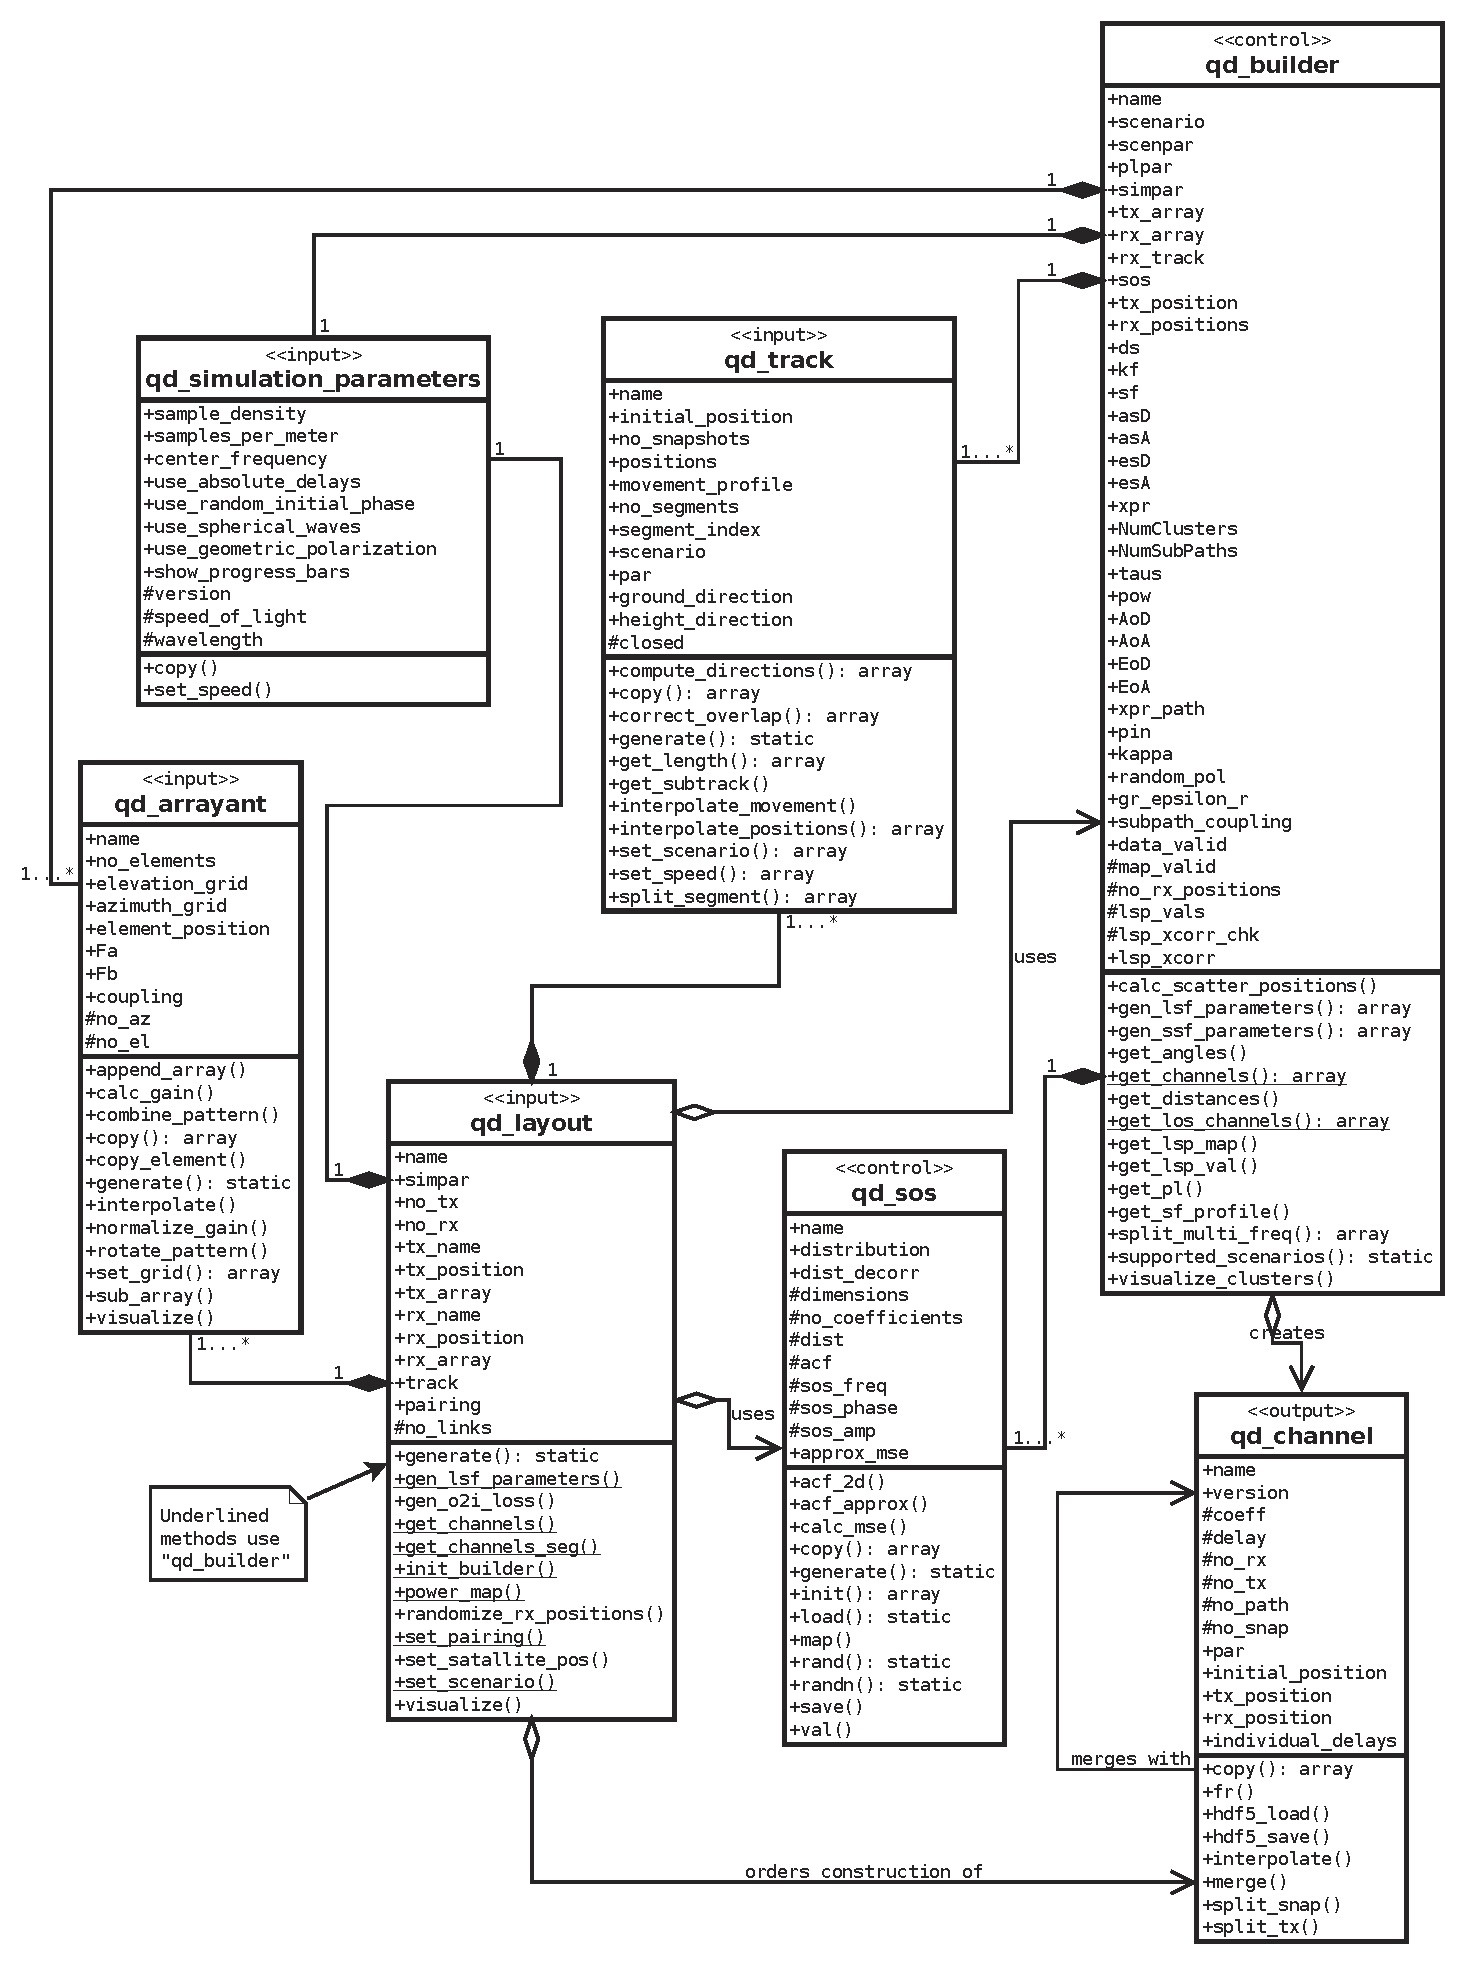
\includegraphics[width=\linewidth]{imagenes/uml_quadriga.png}
	\caption{Diagrama de clases UML de QuaDRiGa.}
	\label{fig:uml_quadriga}
\end{figure}

% Pasos de uso

Cada simulación en \textit{QuaDRiGa} está hecha en tres pasos más un cuarto paso opcional, obteniendo como resultado un objeto de la clase \textit{qd\_channel}:

\begin{enumerate}
    \item Configurar escenario. Esto conlleva la declaración de objetos de las cuatro clases que se toman como entrada, los cuales modelan antenas -tanto para receptor como emisor, para lo cual \textit{QuaDRiGa} ya incluye sus propios modelos predeterminados-, seguimiento de terminales móviles -especificando patrón de movimiento, distancia recorrida, etc.-, escenarios para terminales y/o estaciones base y, por último, capas de simulación que, como se mencionó anteriormente, están caracterizados por parámetros como frecuencia de trabajo, posiciones de estaciones base o emparejamientos entre estaciones base y terminales.
    \item Generar parámetros de gran escala correlados. Esto se hace mediante el uso de la clase \textit{qd\_sos} que a través de los parámetros extraídos de la base de datos de canales que integra \textit{QuaDRiGa}, genera señales aleatorias a través del método de suma de sinusoides.
    \item Calcular los coeficientes de canal fusionados y correlados a través de la clase \textit{qd\_builder} que unifica todos los objetos de entrada más las señales generadas en el paso número 2 para obtener coeficientes de canal representados mediante sus amplitudes, desfases y otros parámetros como ángulos de llegada. Además, se ofrece la opción de obtener dichos coeficientes en dominio de la frecuencia para posibles procesados posteriores.
    \item Post-procesado (opcional). Dentro de los procesados posteriores, más allá del método que implementa la clase dedicada a los canales, no existen más herramientas que permitan obtener resultados más representativos o concluyentes sobre la simulación. Por ello, en este cuarto paso es donde se centra la labor de desarrollo del simulador, como se verá en el Capítulo \ref{cap.implementacion}.
\end{enumerate}

\subsection{Capacidades y limitaciones. Demostración práctica}

Una vez que se adquiere una visión general sobre \textit{QuaDRiGa}, su uso y los conceptos que engloba, es posible realizar un uso estándar del mismo. En esta sub-sección se realizará un ejemplo de simulación utilizando únicamente \textit{QuaDRiGa} con la finalidad de plasmar sus funcionalidades y sus carencias, de modo que podrá ser comparado con futuros ejemplos de uso de \textit{5Gneralife}.

En primer lugar, señalar su uso exclusivo mediante línea de comandos y/o \textit{scripts}, lo cual puede resultar abstracto para un usuario que comience a usar \textit{QuaDRiGa}, especialmente en casos en los que dicho usuario nunca antes haya realizado una toma de contacto con un simulador de comunicaciones móviles.

Como solamente se puede controlar por línea de texto, para este ejemplo se ha desarrollado un \textit{script} que pretende simular una capa de simulación para un entorno de macro-celdas completamente urbano. Dicha capa contará con 10 receptores en movimiento, recorriendo cada uno 1 km. Además, se incluirá un total de tres estaciones base. Tanto terminales como estaciones base tendrán una posición aleatoria y sus antenas serán omnidireccionales de ganancia 5 dBi para simplificaciones. La frecuencia de trabajo será de 2,6 GHz.

Para la puesta en marcha del escenario, el primer paso es la configuración de parámetros de simulación, tarea que solamente precisa de crear un objeto de la clase \textit{qd\_simulation\_parameters} y modificar su atributo de frecuencia a 2,6 GHz:

\begin{lstlisting}[style=Matlab-editor, basicstyle=\tiny]
%% Parametros de simulacion
sim_param = qd_simulation_parameters; % Se genera un objeto de parametros
sim_param.center_frequency = 2.6e9;   % Frecuencia de 2,6 GHz
\end{lstlisting}

A continuación, se hace el proceso análogo para crear dos objetos de la clase \textit{qd\_arrayant} que modelarán sendas antenas omnidireccionales, una para cada tipo de elemento de la simulación -terminales y estaciones base-:

\begin{lstlisting}[style=Matlab-editor, basicstyle=\tiny]
%% Antenas
antenaMT = qd_arrayant('omni'); % Asignacion de antena omnidireccional de ganancia 5 dBi
antenaBS = qd_arrayant ('omni');
\end{lstlisting}

Acto seguido, se realiza la elaboración de la capa de simulación. Como en este caso no existe más de un tipo de celda ni más de una frecuencia, solo es necesario crear una capa. La capa integra los datos sobre estaciones base y receptores, así como el tipo de entorno. En primer lugar se crea el objeto y se configuran los emisores y receptores con el número de cada uno de ellos y sus corresponientes antenas:

\begin{lstlisting}[style=Matlab-editor, basicstyle=\tiny]
%% Transmisores y receptores

layout_uma = qd_layout(sim_param); % Generamos capa de simulacion
layout_uma.no_tx = 3; % 3 estaciones base
layout_uma.no_rx = 10; % 10 usuarios

layout_uma.rx_array = antenaMT; % Asignacion de antena de terminal
layout_uma.tx_array = antenaBS; % Asignacion de antena de BS
\end{lstlisting}

Acto seguido, se configuran las posiciones de los mismos. Para ello se hace uso del método \textit{randomize\_rx\_positions} para los receptores, y un pequeño bucle \textit{for} para los transmisores. Se ha decidido que la distancia máxima del centro a la que pueden estar los elementos sea de 2 km:

\begin{lstlisting}[style=Matlab-editor, basicstyle=\tiny]
%% Posiciones
% Posiciones de usuarios aleatorias con altura de 1,5 m:
layout_uma.randomize_rx_positions(2000, 1.5, 1.5, 0); 

% Posiciones de Bs aleatorias:
for i = 1:layout_uma.no_tx
    pos_x = randi(4000) - 2000; % Posicion X aleatoria entre -2000 y 2000 m del centro
    pos_y = randi(4000) - 2000; % Posicion Y aleatoria entre -2000 y 2000 m del centro
    altura = 25; % 25 metros de altura
    layout_uma.tx_position(:, i) = [pos_x, pos_y, altura];
end
\end{lstlisting}

Para completar la configuración de la capa, es necesario modelar los dos últimos aspectos del escenario: el entorno y el movimiento de los usuarios. Para el movimiento, se ha utilizado un modelado de calle que \textit{QuaDRiGa} implementa, con una orientación aleatoria entre 0 y 360 grados, una longitud mínima de 50 m para las calles, una media de longitud de calle de 187 m, una desviación típica de 83 metros para su longitud, un radio de curva de 10 metros para los giros y una probabilidad de girar en un cruce de 0,5 -según la documentación de \textit{QuaDRiGa} es la son los datos obtenidos para modelar las calles de Berlín-. Para el tipo de entorno, se utiliza el método \textit{set\_scenario} tanto para el objeto de \textit{layout} como para cada uno de los objetos \textit{track}, especificando un tipo de entorno de acuerdo al estándar de macro-celda urbana especificado por 3GPP-3D \cite{3gpp3d}, con una probabilidad de visión directa de 0,2, extraído del mismo:

\begin{lstlisting}[style=Matlab-editor, basicstyle=\tiny]
%% Modelado del escenario
NLOS_prob = 0.8; % Probabilidad de NLOS de 80%
layout_uma.set_scenario('3GPP_3D_UMa',[],[]); % Asignacion de macro-celda segun 3GPP-3D

% Generamos movimientos para los usuarios con modelado de calle de Berlin
trk = cell(1);
for a = 1 : layout_uma.no_rx
    trk{1} = qd_track('street', 1000, randi(360), 50, 187, 83, 10, 0.5); % Calle
    trk{1}.initial_position = layout_uma.rx_position(:,a); % Posicion de acuerdo a la inicial
    trk{1}.name = layout_uma.rx_name{a}; % Se asigna un nombre unico
    escenarios = {'3GPP_3D_UMa_LOS', '3GPP_3D_UMa_NLOS'}; % Se asignan escenarios
    trk{1}.set_scenario( escenarios, [1-NLOS_prob, NLOS_prob], [] ); % Se crean segmentos
    layout_uma.track(1,a) = trk{1}.copy; % Se asigna a la capa
end

\end{lstlisting}

Para obtener las variables de salida, el único paso que queda es el de crear un objeto de la clase \textit{qd\_builder} con la finalidad de generar efectos de pequeña escala y finalmente, generar los coeficientes de canal y unirlos para que entre ellos exista correlación. Cabe destacar que el hecho de generar los efectos de pequeña escala aumenta considerablemente el tiempo de ejecución pero permite tener una simulación sustancialmente más realista.

\begin{lstlisting}[style=Matlab-editor, basicstyle=\tiny]
%% Generamos canales
builder = layout_uma.init_builder; % Objeto builder para pequena escala
gen_ssf_parameters( builder ); % Generamos efectos de pequena escala
canales = get_channels( builder ); % Generamos coeficientes de canal
canales_finales = merge( canales );
\end{lstlisting}

Por último, se puede visualizar la capa a través del método que \textit{QuaDRiGa} ofrece, obteniendo como resultado una representación como la de la Figura \ref{fig:repres_ejemplo}.

\begin{lstlisting}[style=Matlab-editor, basicstyle=\tiny]
%% Visualizacion
layout_uma.visualize([],[],2);
\end{lstlisting}

\begin{figure}[h!]
	\centering
    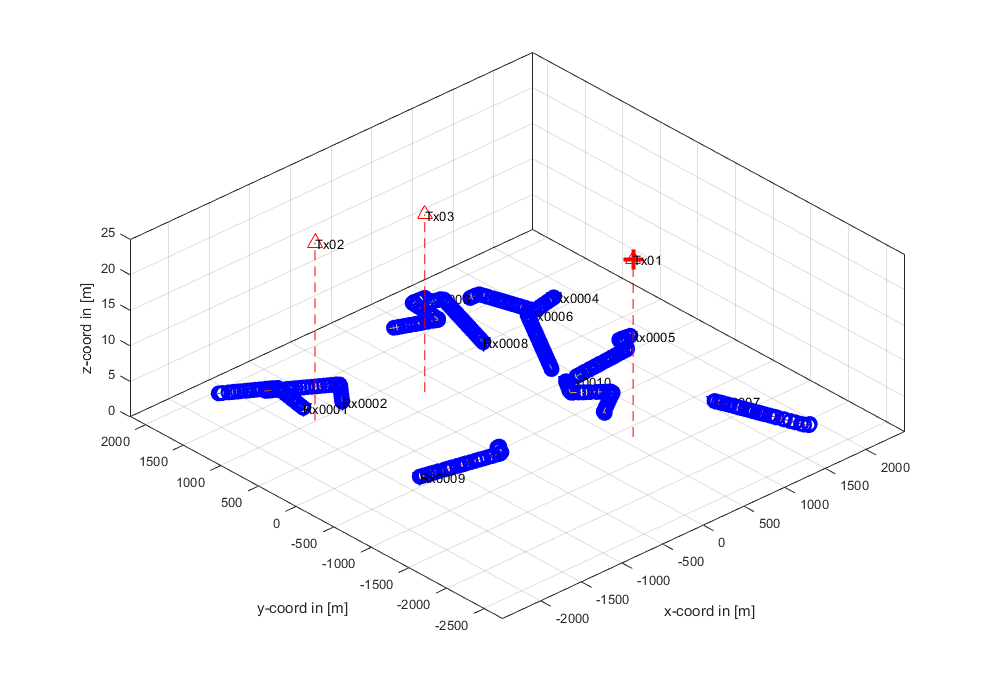
\includegraphics[width=\linewidth]{imagenes/visualizacion_ejemplo.png}
	\caption{Visualización del entorno simulado proporcionada por \textit{QuaDRiGa}.}
	\label{fig:repres_ejemplo}
\end{figure}

Como se observa en la Figura \ref{fig:repres_ejemplo}, se trata de una representación en tres dimensiones que resulta bastante simple a la vez que no detalla ciertos aspectos. Las líneas rojas representan las estaciones base mientras que el cúmulo de puntos es el modo que tiene \textit{QuaDRiGa} de mostrar las trayectorias de sus receptores en movimiento. Si ampliamos la zona de uno de los receptores, se puede diferenciar la línea del recorrido mientras que cada uno de los círculos azules representa un cambio de segmento. En cada transición de segmento se asigna un escenario aleatorio con probabilidad 0.2 para LOS y 0.8 para NLOS. Véase la Figura \ref{fig:receptor_ejemplo}.

\begin{figure}[h!]
	\centering
    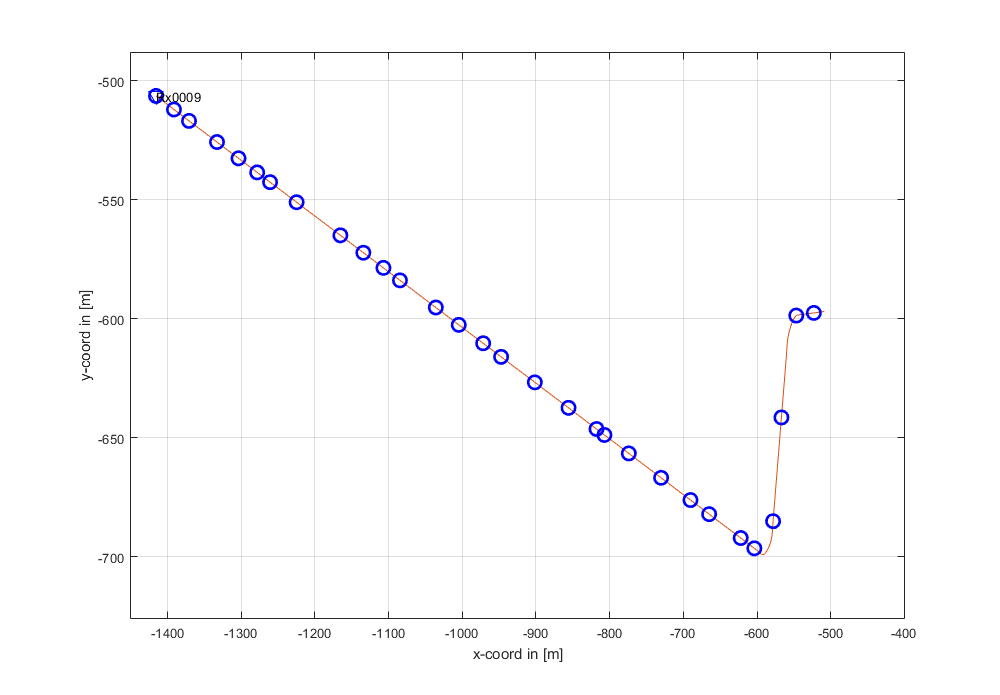
\includegraphics[width=\linewidth]{imagenes/visualizacion_ejemplo_rx1.png}
	\caption{Visualización del recorrido de uno de los receptores.}
	\label{fig:receptor_ejemplo}
\end{figure}

Además, resulta interesante efectuar una indagación en el objeto de la clase \textit{qd\_channel} que se ha generado como salida. Para empezar, la variable \textit{canales\_finales} es un \textit{array} de celdas que cuenta con unas dimensiones de 1x30. Existe un objeto de tipo canal para cada uno de los posibles enlaces, esto es, para cada uno de los 10 receptores, existen 3 objetos de canal, uno `por cada estación base.

Si se abren los datos de uno de los 30 canales, se puede observar la composición del mismo, como muestra la Figura \ref{fig:variable_canal}:

\begin{figure}[h!]
	\centering
    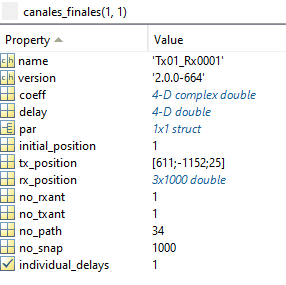
\includegraphics{imagenes/canal_generado_ejemplo.PNG}
	\caption{Estructura de un objeto de la clase \textit{qd\_channel} generado en el ejemplo.}
	\label{fig:variable_canal}
\end{figure}

En primer lugar, se aprecia el nombre del canal que hace referencia a los dos elementos que constituyen el enlace, el transmisor número 1 -Tx01- y el receptor número 1 -Rx01-. Entre los atributos de interés se encuentran las variables \textit{coeff} y \textit{delay}, dos matrices de dimensiones 1x1x34x1000 -dimensiones correspondientes al número de receptores, el número de emisores, el número de trayectorias que el rayo de la señal ha tomado, y el número de posiciones del receptor a través de su recorrido- que contienen las amplitudes y las fases de los coeficientes de canal generados, normalizados. Estos datos a priori no proporcionan información tangible para simulaciones, por lo que es tarea de un simulador basado en \textit{QuaDRiGa} la de procesar posteriormente estos canales con la finalidad de extraer información y obtener datos de caracterización específicos, como podría ser la capacidad del canal.

Como dato a tener en cuenta, el proceso de la simulación de este ejemplo tomó un tiempo de ejecución de 209,25 segundos -3 minutos y medio aproximadamente- utilizando un ordenador de las características que aparecían en la Tabla \ref{tab:caracteristicas}, por lo que es de esperar que para simulaciones más complejas, sean necesarias unas capacidades computacionales considerables.

Para concluir y a modo de resumen, mencionar que para ilustrar el funcionamiento de \textit{QuaDRiGa} con un ejemplo, se ha configurado una entrada compuesta por la generación de objetos que han parametrizado los detalles de la simulación -como por ejemplo la frecuencia de trabajo-. También la capa de simulación incluyendo en ella el número de terminales y su movimiento, el número de estaciones base y su posición, así como el entorno de simulación -en concreto, se ha optado por el modelo 3D de 3GPP publicado en el informe técnico 36.873-. Por otro lado, como salida se ha obtenido un objeto de la clase \textit{qd\_channel}, cuya arquitectura permite obtener las amplitudes normalizadas y las fases de la señal de enlace entre cada uno de los terminales y las estaciones base. También se ha podido obtener una representación visual de la capa de simulación (Figura \ref{fig:esquema_ejemplo}).

% Figura de un esquema
\begin{figure}[ht!]
	\centering
    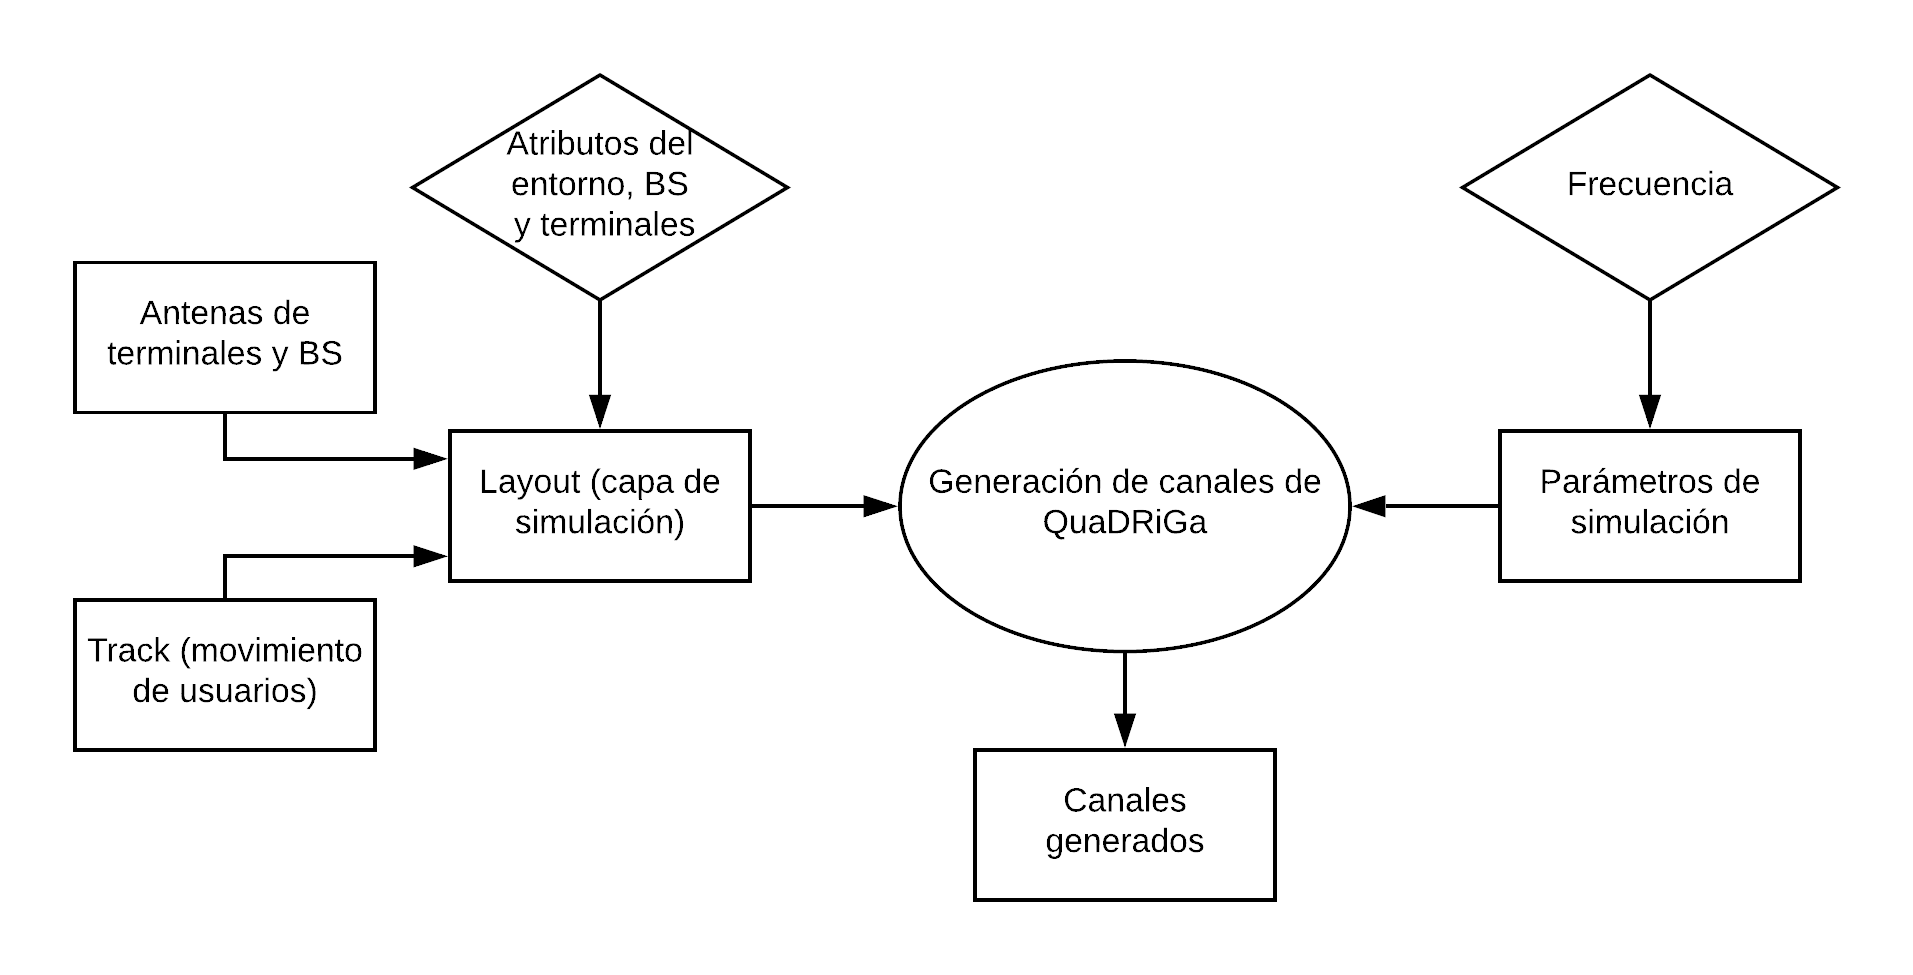
\includegraphics[width=\linewidth]{imagenes/diagrama_ejemplo.png}
	\caption{Diagrama de utilización de \textit{QuaDRiGa}.}
	\label{fig:esquema_ejemplo}
\end{figure}

Si bien estos parámetros de salida son los más dificultosos de obtener debido a su complejidad de cómputo y a la estricta normativa de estándares por los que se rige, no son suficientes y necesitan un procesado extenso para la obtención de datos propios de un simulador. Por ello, el reto que se plantea para implementar un simulador a partir de \textit{QuaDRiGa} como el que se ha desarrollado para este Trabajo de Fin de Grado es el de un código que, de por sí solo, sea capaz de generar e interpretar coeficientes de canal que surjan a partir de configuraciones específicas de 5G, incluyendo, entre otras, funcionalidades de creación de celdas de distinta naturaleza, compartir los mismos usuarios entre todas las capas de simulación -algo que no es posible con \textit{QuaDRiGa}-, obtención de visualizaciones mejoradas y cálculo de parámetros característicos de salida que permitan evaluar objetiva y fácilmente la red creada.

